
\documentclass[11pt,a4paper]{article}

\usepackage[utf8]{inputenc}
\usepackage[T1]{fontenc}
\usepackage[margin=1in]{geometry}
\usepackage{lmodern}
\usepackage{microtype}
\usepackage{graphicx}
\usepackage{xcolor}
\usepackage{hyperref}
\usepackage{booktabs}
\usepackage{longtable}
\usepackage{array}
\usepackage{amsmath,amssymb}
\usepackage{fancyhdr}
\usepackage{caption}
\usepackage{subcaption}
\usepackage{natbib}
\usepackage{tikz}
\usetikzlibrary{positioning, arrows.meta, shapes.geometric, fit}
\usepackage{listings}

\definecolor{accent}{HTML}{1D4ED8}
\definecolor{softblue}{HTML}{EFF6FF}
\definecolor{softgray}{HTML}{F7F7F7}
\definecolor{linegray}{HTML}{D1D5DB}
\definecolor{codebackground}{HTML}{F5F5F5}
\definecolor{codekeyword}{HTML}{1D4ED8}
\definecolor{codecomment}{HTML}{166534}

\hypersetup{
    colorlinks=true,
    linkcolor=accent,
    urlcolor=accent,
    citecolor=accent,
    pdftitle={A Dual-Precision MX Datapath for Layer-Adaptive RLHF Quantization on FPGAs},
    pdfauthor={Hiva Zaad, Danny Adkins, Grant Griffith}
}

\lstdefinestyle{codestyle}{
    backgroundcolor=\color{codebackground},
    basicstyle=\ttfamily\small,
    keywordstyle=\color{codekeyword}\bfseries,
    commentstyle=\color{codecomment}\itshape,
    breaklines=true,
    keepspaces=true,
    frame=single,
    framerule=0.4pt,
    rulecolor=\color{black!20},
    xleftmargin=0.7em,
    xrightmargin=0.4em,
    aboveskip=0.8em,
    belowskip=0.6em,
}
\lstset{style=codestyle}

\captionsetup{font=small, labelfont=bf}
\setlength{\parskip}{0.35em}
\setlength{\parindent}{0pt}
\renewcommand{\arraystretch}{1.15}
\pagestyle{fancy}
\fancyhf{}
\fancyhead[L]{\small CS217 Final Project}
\fancyhead[R]{\small Layer-Adaptive MX Quantization for RLHF}
\fancyfoot[C]{\thepage}
\renewcommand{\headrulewidth}{0.4pt}

\newcolumntype{L}[1]{>{\raggedright\arraybackslash}p{#1}}
\newcolumntype{C}[1]{>{\centering\arraybackslash}p{#1}}

\graphicspath{{figures/}}

\begin{document}

\begin{center}
    {\LARGE \textbf{A Dual-Precision MX Datapath for Layer-Adaptive\\
    RLHF Quantization on FPGAs}}\\[0.9em]
    {\large Stanford CS217 Hardware Accelerators Project}\\[1.2em]

    \begin{tabular}{cc}
        \begin{tabular}{c}
            \textbf{Hiva Zaad (Mohammadzadeh)}\\
            Department of Computer Science\\
            Stanford University\\
            \texttt{hiva@stanford.edu}
        \end{tabular}
        &
        \begin{tabular}{c}
            \textbf{Danny Adkins}\\
            Graduate School of Business\\
            Stanford University\\
            \texttt{dadkins@stanford.edu}
        \end{tabular}
    \end{tabular}\\[0.8em]

    \begin{tabular}{c}
        \textbf{Grant Griffith}\\
        Graduate School of Business\\
        Stanford University\\
        \texttt{grgriff@stanford.edu}
    \end{tabular}\\[0.8em]

    \small \textbf{Code:} \url{https://github.com/HivaMohammadzadeh1/CS217-Final-Project}\\
    \small \textbf{Dataset:} \url{https://huggingface.co/datasets/hivamoh/cs217-rlhf-dataset}
\end{center}

% ══════════════════════════════════════════════════════════
\begin{abstract}
Reinforcement learning from human feedback (RLHF) is expensive because each PPO step runs rollout, reward, and gradient phases over the same transformer, but those phases do not need the same numerical precision. We study whether an FPGA accelerator can exploit that fact with runtime-selectable microscaling (MX) formats.

Our target workload is Qwen2.5-0.5B on Anthropic HH-RLHF, integrated with a host-managed tiled offload path on AWS F2. We first measure the deployed INT8 baseline and find that the current 16x16 tile launch path is dominated by off-chip overhead: 148,641 of 148,656 measured cycles per tile sit in host-side launch, PCIe, and AXI movement, while the PE itself accounts for 15 cycles. That imbalance is a property of this tiny-tile prototype, but it makes compression the most immediate lever. We then profile all 169 quantizable layers under MXFP4 and MXFP8. MXFP8 is safe everywhere. MXFP4 is safe for 158 of 169 layers, while failures cluster in early and late MLP blocks and in the LM head.

Guided by these results, we build a dual-precision SystemC datapath with explicit mode switching and flush semantics, then carry the same contract into the HLS design. The MX-capable bitstream has not yet been re-synthesized and deployed, so we report hardware numbers for the INT8 baseline, SystemC accuracy for MX arithmetic, and conservative policy-level projections for end-to-end RLHF. Under the current bandwidth-dominated interface, a balanced policy that uses MXFP4 on the tolerant subset is projected to cut transferred bytes by about 40\% and FPGA energy by about 20\%.
\end{abstract}

\medskip
\noindent\fbox{\parbox{\dimexpr\linewidth-2\fboxsep-2\fboxrule}{%
\textbf{Scope of evaluation.}
Hardware measurements come from the deployed INT8 AWS F2 baseline. Layer sensitivity comes from PyTorch plus \texttt{mx-pytorch}. MX arithmetic, mode switching, and datapath correctness come from the SystemC reference model. End-to-end MX energy savings are still projections because the MX RTL has been integrated into the HLS path but has not yet been re-synthesized into a deployable AFI.}}
\medskip

% ══════════════════════════════════════════════════════════
\section{Introduction}

RLHF is now the standard way to align large language models with human preferences \citep{ouyang2022training, christiano2017deep}. It is also an awkward workload for hardware. A single PPO step mixes three very different phases. Rollout is mostly autoregressive sampling. Reward scoring is inference that collapses a long hidden-state trajectory into one scalar. Gradient updates are numerically fragile because many small errors can accumulate across steps. Treating all three phases as if they need the same precision leaves efficiency on the table.

FPGAs are attractive here for one simple reason: they let us build the exact numerical path we want. We can decode custom formats, choose where to spend bits, and switch modes at runtime without paying GPU-style overhead for unused tensor-core functionality. But that only helps if the format change attacks the real bottleneck.

Our first result is that the deployed CS217 baseline is not compute-bound in its current form. The present 16x16 tile launch path spends almost all of its measured cycles outside the PE, in launch and movement overhead. That changes the design question. The first lever to pull is not a faster multiply-accumulate unit. It is a format that reduces transferred bytes while keeping model quality intact.

Microscaling formats \citep{rouhani2023mxformat} are a good fit for that problem. They preserve dynamic range with group scaling, but they use fewer bits per value than FP16. The project therefore asks a narrow hardware question: can we assign MXFP8 and MXFP4 at layer and phase granularity, route those choices through a usable software interface, and build a datapath that supports the policy safely?

This paper makes four contributions.

\begin{enumerate}    \item We characterize the deployed AWS F2 baseline and show that transfer, not arithmetic, dominates the current offload path.
    \item We profile all 169 quantizable layers in Qwen2.5-0.5B and identify the exact layers that fail MXFP4 tolerance.
    \item We design and validate a dual-precision SystemC datapath with safe runtime mode switching, then map the same contract into the HLS design.
    \item We use the measured bottleneck and the learned sensitivity map to build conservative RLHF policy projections for end-to-end energy reduction.
\end{enumerate}


% ══════════════════════════════════════════════════════════
\section{Background and Related Work}
\label{sec:related-work}

\paragraph{RLHF Training}
Reinforcement learning from human feedback~\citep{ouyang2022training, christiano2017deep} has emerged as the dominant paradigm for aligning language models with human preferences.
The approach first trains a reward model on pairwise preference data, then uses this reward signal to optimize the policy via Proximal Policy Optimization~\citep{schulman2017ppo}.
Each PPO iteration generates responses from the current policy, scores them with the reward model, and computes gradients to improve future generations.
The TRL library~\citep{vonwerra2022trl} provides the standard PyTorch implementation we build upon.

\paragraph{Microscaling Formats}
The MX format family~\citep{rouhani2023mxformat} introduces block-scaled numerical representations designed for deep learning workloads.
Rather than storing a full exponent per element, MX formats share a single scale factor across groups of $k$ values (typically 8 or 16), reducing storage while preserving dynamic range.
MXFP8 uses 8-bit elements (E4M3: 4-bit exponent, 3-bit mantissa) and matches FP16 quality on most inference tasks.
MXFP4 uses 4-bit elements (E2M1: 2-bit exponent, 1-bit mantissa), halving bandwidth at the cost of reduced precision.
Microsoft's \texttt{mx-pytorch} library provides reference implementations for quantization and dequantization.

\begin{figure}[t]
\centering
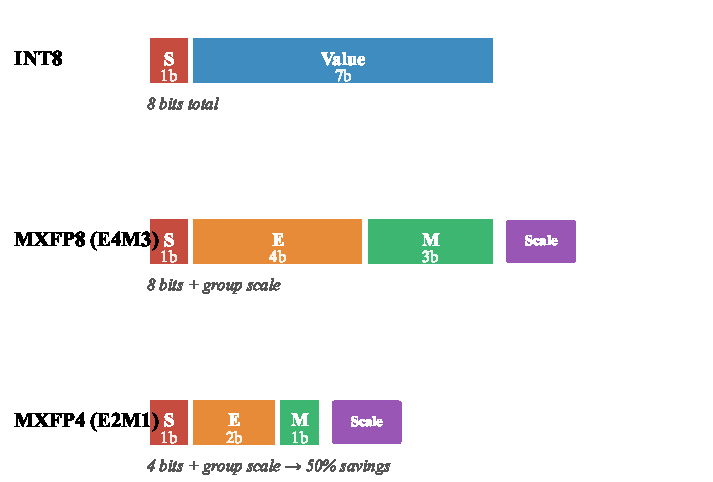
\includegraphics[width=0.85\linewidth]{mx_format_comparison.pdf}
\caption{Bit layouts for INT8, MXFP8, and MXFP4. MX formats share a group scale factor across multiple elements, enabling aggressive bit-width reduction while maintaining dynamic range.}
\label{fig:mx-formats}
\end{figure}

\paragraph{Low-Precision Training}
Mixed-precision training with FP16~\citep{micikevicius2018mixed} is now standard practice, and recent work extends this to FP8~\citep{micikevicius2022fp8}.
NVIDIA's H100 provides native FP8 tensor cores, demonstrating industry momentum toward lower precision.
However, sub-8-bit training remains challenging because gradient accumulation amplifies quantization errors.
Our work sidesteps this limitation by applying aggressive quantization selectively---only to phases and layers that can tolerate it.

\paragraph{FPGA Acceleration}
FPGAs offer energy-efficient matrix multiplication through custom datapaths and flexible precision~\citep{guo2017angel, wang2021fpga}.
The AWS F2 platform provides cloud-accessible Xilinx VU9P FPGAs with PCIe Gen3 x16 connectivity.
We extend the CS217 Lab~1 INT8 processing element with MX format support.

\paragraph{Adaptive Quantization}
Prior work on mixed-precision quantization~\citep{dong2019hawq, wang2019haq} uses Hessian eigenvalues or learned policies to assign per-layer bit widths for inference.
Our work differs in three ways: we target RLHF training rather than inference, we exploit phase-specific tolerance within the training loop, and we use MX group scaling rather than per-tensor quantization.


% ══════════════════════════════════════════════════════════
\section{Problem Definition and FPGA Motivation}

\subsection{Target workload}

The target application is PPO-based RLHF on Qwen2.5-0.5B-Instruct \citep{qwen2025qwen25} using Anthropic HH-RLHF \citep{bai2022training} and the TRL software stack \citep{vonwerra2022trl}. Each transformer block contains seven major linear projections: Q, K, V, O, gate, up, and down. Including the LM head, this gives 169 quantizable layers for sensitivity analysis.

The project does \emph{not} attempt to move the full RLHF stack onto FPGA. Tokenization, sampling, KL computation, optimizer logic, and all host orchestration stay in PyTorch. The accelerator target is the tiled linear-algebra kernel inside those layers. That choice is deliberate: it gives us a realistic software-hardware split and lets the accelerator follow workload structure instead of pretending the entire RLHF loop is one monolithic kernel.

\begin{table}[h!]
\centering
\small
\begin{tabular}{L{4.1cm}L{8.2cm}}
\toprule
\textbf{Item} & \textbf{Value} \\
\midrule
Policy / reward model & Qwen2.5-0.5B-Instruct \\
RLHF algorithm & PPO via TRL \\
Dataset & Anthropic HH-RLHF subset, 1,000 train and 200 eval examples \\
Sequence budget & Up to 512 tokens \\
Quantizable layers profiled & 169 (24 blocks $\times$ 7 projections, plus LM head) \\
Deployed hardware kernel & CS217 Lab 1 INT8 tiled kernel on AWS F2 \\
Current software-hardware split & Host runs RLHF control flow; FPGA offloads selected tiled linear ops \\
Primary optimization target & Reduce transferred bytes and FPGA energy while preserving reward and perplexity \\
\bottomrule
\end{tabular}
\caption{Target workload and project scope.}
\label{tab:workload-summary}
\end{table}

At tile granularity, the current kernel is intrinsically low-intensity. One 16\(\times\)16 weight tile times one 16-element input tile performs 256 MACs while moving 336 bytes, which is only 0.76 MAC per byte, or 1.52 arithmetic operations per byte if multiply and add are counted separately. That is a poor trade unless tiles are batched and reused. It is the main reason the paper treats burst structure, buffering, and weight residency as design issues rather than bookkeeping.

One important constraint is that the deployed path is still selective. In the real 50-step hardware run, the project offloads all reward-model attention projections and a small set of policy-model attention projections, while gradient-phase computation remains in PyTorch because the current path is not autograd-safe. This is enough to validate the accelerator interface and collect real hardware numbers, but it also means the final policy results are projections rather than a completed MX deployment.

\subsection{Why FPGA for this problem}

An FPGA is a good fit here for three workload-specific reasons.

First, the workload needs custom precision rather than generic floating-point throughput. MXFP8 and MXFP4 require explicit decode logic, shared group-scale handling, and controlled mode switching. Those are natural FPGA tasks.

Second, RLHF phase structure creates a real use case for runtime-selectable datapaths. A fixed low-precision accelerator would be too brittle. A runtime-selectable datapath can choose aggressive compression in rollout, safer compression in reward, and higher precision in gradient.

Third, the deployed baseline is bandwidth-limited. In that setting, FPGAs let us attack bytes directly. We can reshape the on-wire representation, not just the arithmetic inside the PE. That is the main reason MX is interesting in this project.

\subsection{Evaluation scope}

Table~\ref{tab:evidence-boundary} separates direct measurements, SystemC validation, and end-to-end projections.

\begin{table}[h!]
\centering
\small
\begin{tabular}{L{3.2cm}L{4.5cm}L{4.2cm}}
\toprule
\textbf{Claim type} & \textbf{Source} & \textbf{Used for} \\
\midrule
Hardware baseline & AWS F2 INT8 bitstream at 250 MHz & Tile latency, transfer bottleneck, phase timing, sanity-check RLHF run \\
Layer sensitivity & PyTorch + \texttt{mx-pytorch} profiling & Which layers are safe in MXFP4 or need MXFP8 fallback \\
Datapath correctness & SystemC testbench and HLS-compatible reference behavior & Quantization fidelity, MAC/GEMM error, flush-on-switch safety \\
End-to-end MX savings & First-order projection from the measured baseline and learned policy map & Relative policy comparison only \\
\bottomrule
\end{tabular}
\caption{Sources of evidence used in the evaluation.}
\label{tab:evidence-boundary}
\end{table}


% ══════════════════════════════════════════════════════════
\section{Accelerator Design}

\subsection{Programming model and software mapping}

The software-visible contract is simple on purpose. The host chooses a tile, names the layer and RLHF phase, selects a precision mode from the policy map, and launches the tile through the existing PE configuration path. A mode change is not implicit. The caller must request the new mode and flush before issuing work.

\begin{lstlisting}[language=Python, caption={Host-side targeting model for one tiled linear op.}, label={lst:api}]
mode = controller.select(phase="rollout", layer_id=layer_id)
fpga.configure_precision(mode=mode, group_size=8)
fpga.flush_pipeline()
y_tile = fpga.matmul(x_tile, w_tile)
\end{lstlisting}

That contract gives the accelerator a usable programming model rather than a paper-only policy. It also makes the safety rule explicit. If software changes from INT8 to MXFP8 or MXFP4, the datapath must be drained before the next tile enters.

\begin{table}[h!]
\centering
\small
\begin{tabular}{L{3.4cm}L{8.3cm}}
\toprule
\textbf{Parameter class} & \textbf{Examples} \\
\midrule
Compile-time constants & tile size 16\(\times\)16, vector width 16 bytes, supported modes \{\texttt{INT8}, \texttt{MXFP8}, \texttt{MXFP4}\}, supported group sizes \{8, 16\} \\
Runtime control & layer id, RLHF phase, precision mode, group size flag, tile addresses, PE configuration fields \\
Software-visible constraints & dimensions must be padded or tiled to kernel shape, mode changes require \texttt{flush\_pipeline()}, deployed autograd path still falls back to host FP16 for gradient updates \\
\bottomrule
\end{tabular}
\caption{Compile-time and runtime parameters exposed by the programming model.}
\label{tab:programming-model}
\end{table}

\begin{figure}[t]
\centering
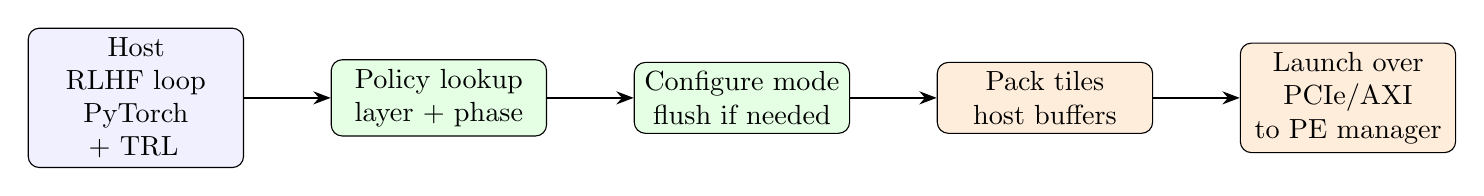
\begin{tikzpicture}[
    node distance=0.75cm and 1.1cm,
    box/.style={rectangle, draw, rounded corners, minimum height=0.88cm, text width=2.5cm, align=center},
    host/.style={box, fill=blue!6},
    ctl/.style={box, fill=green!10},
    hw/.style={box, fill=orange!14},
    arr/.style={-{Stealth[length=2.2mm]}, thick}
]
\node[host] (host) {Host RLHF loop\\PyTorch + TRL};
\node[ctl, right=of host] (policy) {Policy lookup\\layer + phase};
\node[ctl, right=of policy] (cfg) {Configure mode\\flush if needed};
\node[hw, right=of cfg] (pack) {Pack tiles\\host buffers};
\node[hw, right=of pack] (fpga) {Launch over PCIe/AXI\\to PE manager};

\draw[arr] (host) -- (policy);
\draw[arr] (policy) -- (cfg);
\draw[arr] (cfg) -- (pack);
\draw[arr] (pack) -- (fpga);
\end{tikzpicture}
\caption{Software-visible launch path. The host selects a mode from the per-layer policy, writes the corresponding configuration fields, flushes on mode changes, then launches the tile through the existing PCIe and AXI path.}
\label{fig:system-overview}
\end{figure}

\subsection{PE microarchitecture}

The hardware target is not a monolithic transformer accelerator. It is one precision-selectable processing element built on top of the CS217 PECore structure. The checked-in design keeps the original 16-byte vector width and extends the PE configuration with two MX control fields: precision mode and group-size selection. Internally, the PE is organized around three pieces.

\begin{enumerate}    \item \textbf{Banked local storage.} Weights are held in a 16-bank scratchpad, one bank per logical lane. The checked-in configuration reduces weight read bandwidth to four read ports to ease timing and SRAM port pressure. Input and bias storage are much smaller single-bank structures.
    \item \textbf{Precision-selectable arithmetic.} INT8 tiles follow the original byte-multiply path. MX tiles pass through a decode stage that reconstructs fixed-point values from E4M3 or E2M1 elements plus the shared group scale, then feeds the same product-sum structure.
    \item \textbf{A cycle-level PE control path.} The PE executes a fixed sequence each step: state-machine update, scratchpad access, MAC, scaling, output push, then state update for the next issue.
\end{enumerate}

At the chosen setting, one issue step can consume four vector words from the weight path. Because the 16-element dot-product loops are fully unrolled, that exposes up to \(4 \times 16 = 64\) byte multiplies in parallel inside the arithmetic stage. A full 16-port version would expose 256, but the code deliberately backs off from that point because the memory system becomes the real timing problem.

\begin{figure}[t]
\centering
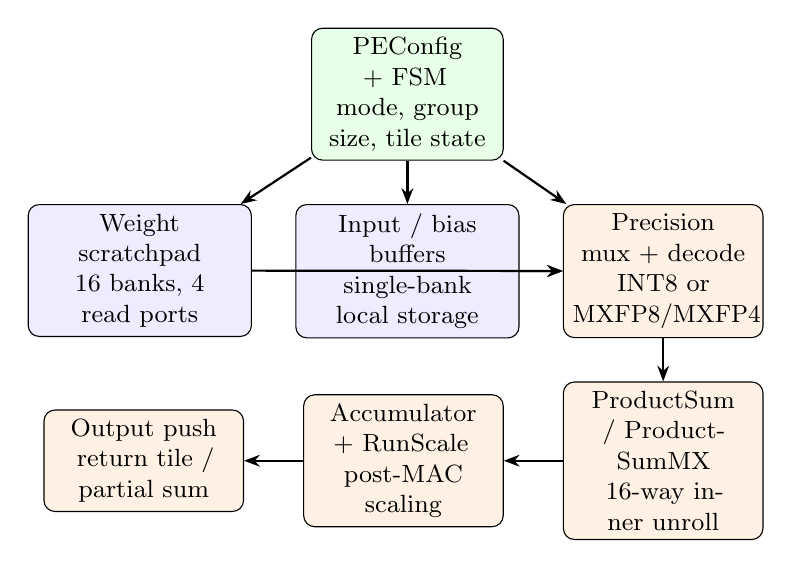
\begin{tikzpicture}[
    node distance=0.55cm and 0.75cm,
    box/.style={rectangle, draw, rounded corners, minimum height=0.82cm, align=center, fill=orange!10, text width=2.3cm},
    mem/.style={rectangle, draw, rounded corners, minimum height=0.82cm, align=center, fill=blue!7, text width=2.6cm},
    ctl/.style={rectangle, draw, rounded corners, minimum height=0.82cm, align=center, fill=green!9, text width=2.2cm},
    arr/.style={-{Stealth[length=2mm]}, thick},
    font=\small
]
\node[ctl] (cfg) {PEConfig + FSM\\mode, group size, tile state};
\node[mem, below left=of cfg] (w) {Weight scratchpad\\16 banks, 4 read ports};
\node[mem, below=of cfg] (x) {Input / bias buffers\\single-bank local storage};
\node[box, below right=of cfg] (dec) {Precision mux + decode\\INT8 or MXFP8/MXFP4};
\node[box, below=of dec] (mac) {ProductSum / ProductSumMX\\16-way inner unroll};
\node[box, left=of mac] (acc) {Accumulator + RunScale\\post-MAC scaling};
\node[box, left=of acc] (out) {Output push\\return tile / partial sum};

\draw[arr] (cfg) -- (w);
\draw[arr] (cfg) -- (x);
\draw[arr] (cfg) -- (dec);
\draw[arr] (w) -- (dec);
\draw[arr] (x) -- (dec);
\draw[arr] (dec) -- (mac);
\draw[arr] (mac) -- (acc);
\draw[arr] (acc) -- (out);
\end{tikzpicture}
\caption{PE-level microarchitecture. The key change relative to the INT8 baseline is the precision-selectable decode path in front of the multiply-accumulate stage, controlled by the same PE configuration structure that already manages tile execution.}
\label{fig:pe-microarchitecture}
\end{figure}

\subsection{MX formats and adaptive precision}

MX formats use a shared scale per group of values instead of a full exponent per element \citep{rouhani2023mxformat}. We use two formats.

\begin{itemize}    \item \textbf{MXFP8 (E4M3)} is the safe mode. It preserves enough range and mantissa bits that it tracks the FP16 baseline closely.
    \item \textbf{MXFP4 (E2M1)} is the aggressive mode. It cuts value storage roughly in half, but it is much more sensitive to wide dynamic range.
\end{itemize}

The default group size is \(k=8\). In the SystemC sweeps, \(k=8\) is consistently as good as or slightly better than \(k=16\), so there is no reason to take the extra numerical risk unless a later implementation proves that the larger grouping materially simplifies the memory path.

\subsection{SystemC correctness contract}

The SystemC model is the golden reference for the MX datapath. It contains the MX type definitions, group-scale encode and decode logic, a precision-selectable multiply-accumulate path, and a wrapper that models mode changes explicitly.

The correctness rule is simple: mode changes are two-step events. Software first requests the new mode, then flushes the pipeline. Until the flush completes, MAC and GEMM calls are illegal. This prevents a partially drained tile from being decoded with the wrong format and gives the HLS path a clean behavioral contract to preserve.

\subsection{HLS-aware design and optimization}

This is where the design had to become more concrete. The checked-in HLS code is not just ``SystemC rewritten in C++.'' It already makes architectural choices that trade off throughput against routing and memory pressure.

First, the arithmetic loops are aggressively exposed to HLS. The inner product-sum loops in both the INT8 and MX paths are fully unrolled, so one issued vector word performs 16 elementwise multiplies in parallel. The top-level datapath loop over vector lanes is also written for full unrolling. That is the right choice because the tile shape is fixed and tiny; leaving those loops rolled would throw away most of the benefit of a custom PE.

Second, the memory system, not the multiplier tree, sets the practical parallelism point. The design could in principle read 16 weight lanes per issue step, but the checked-in PE specification reduces that to four read ports. This is an explicit timing tradeoff. More ports cut tile issue time, but they also increase bank pressure, crossbar complexity, and fanout into the decode and MAC stages. The current design chooses the smaller point in that space to keep the PE synthesizable.

Third, MX decode is kept local to the arithmetic stage. The design does not expand all weights eagerly in memory. It stores compact MX bytes plus group-scale metadata, decodes only the words being consumed, and then feeds the same accumulation path. That choice preserves the bandwidth benefit of MX and avoids replacing a transfer bottleneck with a much larger on-chip storage footprint.

\begin{table}[h!]
\centering
\small
\begin{tabular}{L{2.8cm}C{1.5cm}C{2.0cm}L{3.1cm}L{2.7cm}}
\toprule
\textbf{Design point} & \textbf{Weight read ports} & \textbf{Parallel byte multiplies per issue} & \textbf{Upside} & \textbf{Main risk} \\
\midrule
Wide ideal & 16 & 256 & fewest issue steps per tile & SRAM ports and routing likely dominate \\
Midpoint & 8 & 128 & better throughput with moderate banking pressure & still heavy fanout into decode and MAC \\
Checked-in design & 4 & 64 & far easier timing closure and simpler arbitration & more issue steps per tile \\
\bottomrule
\end{tabular}
\caption{HLS design space for the PE datapath. The current source tree corresponds to the 4-port design point.}
\label{tab:hls-design-space}
\end{table}

We do \emph{not} have a final Catapult report for the MX-capable path, so we cannot honestly report a measured initiation interval, achieved clock, or DSP/LUT count for that variant. What we can report is the intended optimization direction: keep the 16-way inner arithmetic fully exposed, cap memory-side width at the point where banking remains realistic, and treat decode logic as part of the MAC stage rather than a separate wide preprocessing pass.

\subsection{Memory system and data movement}

The memory story needs to be designed, not just observed. The deployed baseline still launches very small tiles one by one, which is why the measured path is dominated by off-chip and launch overhead. The intended MX deployment therefore uses four concrete memory-side ideas.

\begin{enumerate}    \item \textbf{Contiguous host packing.} Tiles from the same layer should be packed into contiguous host buffers so PCIe can issue larger bursts instead of many tiny transfers.
    \item \textbf{Weight-panel residency.} One weight panel should stay on chip while multiple input vectors sweep across it. That converts repeated weight traffic into on-chip reuse.
    \item \textbf{Double buffering.} While the PE consumes the current panel, the next panel should be filled into a second local buffer.
    \item \textbf{Compact on-wire MX representation.} Weights should stay compressed until they are about to be consumed by the decode stage.
\end{enumerate}

Table~\ref{tab:memory-flow} distinguishes the deployed prototype from the intended buffered design.

\begin{table}[h!]
\centering
\small
\begin{tabular}{L{3.4cm}L{4.1cm}L{4.0cm}}
\toprule
\textbf{Stage} & \textbf{Deployed baseline} & \textbf{Intended MX deployment} \\
\midrule
Host packing & single tiles prepared on demand & layer-local tile batches packed contiguously \\
PCIe / AXI & many small launches & burst transfers of tile panels \\
On-chip storage & transient tile buffers & weight-panel residency with double buffering \\
PE input format & INT8 bytes only & compact INT8 or MX bytes plus scale metadata \\
Reuse policy & little to no weight reuse on chip & reuse one panel across many input vectors before eviction \\
\bottomrule
\end{tabular}
\caption{Current versus intended memory flow. The main change is that buffering and reuse become first-class design goals.}
\label{tab:memory-flow}
\end{table}

A simple byte model makes the tradeoff visible. In the current INT8 path, one tile transfer moves 256 bytes of weights, 16 bytes of input, and 64 bytes of output, for 336 bytes total. If a weight tile is reused across \(R\) input vectors, the effective bytes per matmul become
\[
B_{\mathrm{INT8}}(R) = 80 + \frac{256}{R}.
\]
For MXFP4 with group size 8, the 256 weights become 128 payload bytes plus 32 scale bytes if one scale byte is stored per 8-value group. The corresponding effective traffic is
\[
B_{\mathrm{MXFP4}}(R) = 80 + \frac{160}{R}.
\]

\begin{table}[h!]
\centering
\small
\begin{tabular}{C{1.6cm}C{2.2cm}C{2.4cm}C{2.4cm}}
\toprule
\textbf{Reuse \(R\)} & \textbf{INT8 bytes} & \textbf{MXFP4 bytes} & \textbf{Reduction} \\
\midrule
1 & 336 & 240 & 28.6\% \\
8 & 112 & 100 & 10.7\% \\
16 & 96 & 90 & 6.3\% \\
\bottomrule
\end{tabular}
\caption{Effective bytes per matmul under weight reuse. Compression matters most when reuse is low, while caching matters more as reuse rises. The two techniques stack.}
\label{tab:reuse-bytes}
\end{table}

This is the key design implication. In the current prototype, MX helps because reuse is poor and every saved byte matters. In a stronger design, buffering and caching become at least as important as compression. The right memory system does both.

\subsection{Resource realism and timing constraints}

Even without a final MX synthesis report, the checked-in configuration is concrete enough to support a grounded cost estimate.

The weight scratchpad is the largest local structure. It has 16 banks, 256 entries per bank, and stores one 16-byte vector word per entry, which is about 64~KiB of local storage. The input and bias stores are much smaller at roughly 4~KiB each. Before arbitration overhead and metadata, that puts the visible on-chip storage footprint near 72~KiB. As a rough lower bound, that is about 16 BRAM36 equivalents just for the explicitly declared local memories.

The arithmetic side is also easy to bound qualitatively. The chosen 4-port design issues four vector words per step and fully unrolls the 16-byte dot product inside each word, so the active arithmetic width is 64 byte multiplies plus the associated add tree and decode logic. Relative to the INT8 baseline, MX therefore adds decoder hardware and scale handling in front of each active multiply lane. The likely timing risk is not the multipliers themselves. It is the fanout from banked storage into many parallel decode-plus-multiply lanes.

That is why the read-port reduction in the checked-in design is important. The design is already telling us where timing pressure lives. The practical goal for the next synthesis pass is not ``maximize parallelism at all cost.'' It is to keep enough arithmetic exposed to matter while preserving a realistic clock target near the existing 250~MHz baseline.


% ══════════════════════════════════════════════════════════
\section{Experimental Setup}

\subsection{RLHF run configuration}

We use a curated 1,200-example subset of Anthropic HH-RLHF, split into 1,000 train and 200 eval pairs. The main hardware-backed run uses 50 PPO steps on Qwen2.5-0.5B-Instruct. In the deployed configuration, reward-model attention layers are offloaded broadly, while policy-model offload is limited to representative attention projections in blocks 0 and 23. Gradient computation remains in host FP16.

This setup is enough to validate the runtime path and collect real phase timings. It is \emph{not} the final full-policy deployment that the MX controller is designed for.

\subsection{INT8 hardware baseline}

The baseline accelerator is the CS217 Lab 1 INT8 kernel running on AWS F2 with a Xilinx VU9P at 250 MHz. Each tile launch transfers 256 B of weights, 16 B of inputs, and 64 B of outputs. We average the measured cycle count over repeated runs and separate compute cycles from transfer cycles.

For the per-tile energy proxy, we combine the measured latency with a 35 W board-level power estimate from Xilinx Power Estimator. This gives a coarse relative energy model for comparing policies. We do not treat it as a full-board end-to-end power study.

\subsection{Layer sensitivity profiling}

We profile all 169 quantizable layers with Microsoft's \texttt{mx-pytorch} implementation. For each layer $\ell$, we quantize only that layer while leaving all others at the baseline precision, then measure perplexity on a held-out calibration set.

\[
\Delta_\ell = \frac{\mathrm{PPL}_\ell - \mathrm{PPL}_{\mathrm{base}}}{\mathrm{PPL}_{\mathrm{base}}} \times 100.
\]

A layer is marked MXFP4-safe if it stays within a 2\% perplexity delta at group size 8. The same profiler is also used to generate policies A through D automatically.

\subsection{SystemC validation}

The SystemC testbench validates three things:

\begin{itemize}    \item reconstruction fidelity for MX encode/decode,
    \item MAC and 16x16 GEMM accuracy relative to floating-point reference,
    \item safety of mode switching and pipeline flush behavior.
\end{itemize}

We also run larger statistical sweeps over dynamic range, input distribution, and chained GEMM depth. Those experiments are useful because they explain \emph{why} some layers fail MXFP4. In particular, they show that MXFP4 degrades when the activation range gets wide, which matches the boundary-layer sensitivity seen in the model.


% ══════════════════════════════════════════════════════════
\section{Results}

\subsection{The current tile path is launch- and transfer-bound}

Table~\ref{tab:fpga-baseline} and Figure~\ref{fig:cycle-breakdown} summarize the key hardware result. For one 16x16 tile launch in the deployed prototype, 148,641 measured cycles sit outside the PE and only 15 cycles are spent in the PE itself. The on-wire representation, not the MAC array, is therefore the first thing worth optimizing.

\begin{table}[h!]
\centering
\small
\begin{tabular}{L{5.2cm}r}
\toprule
\textbf{Metric} & \textbf{Value} \\
\midrule
Total cycles per tile & 148,656 \\
Off-chip and launch overhead cycles & 148,641 (99.99\%) \\
On-chip PE cycles & 15 (0.01\%) \\
Latency per tile & 594.62~$\mu$s \\
Throughput & 1,682~tiles/s \\
Per-tile energy proxy at 35 W & 20.81~mJ \\
\bottomrule
\end{tabular}
\caption{AWS F2 INT8 baseline for one 16x16 tile launch in the deployed prototype.}
\label{tab:fpga-baseline}
\end{table}

\begin{figure}[t]
\centering
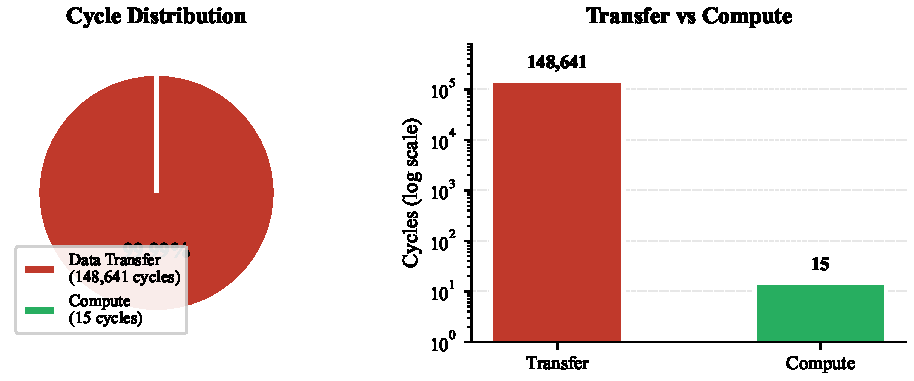
\includegraphics[width=0.96\linewidth]{cycle_breakdown.pdf}
\caption{Cycle breakdown for one 16x16 tile launch in the deployed INT8 prototype. Most cycles are spent in host-device launch and movement overhead rather than in the PE itself.}
\label{fig:cycle-breakdown}
\end{figure}

This observation also explains why MX is attractive even before the full MX AFI exists. If the bottleneck were DSP throughput, then lower precision would only matter if it let us instantiate more parallel MACs. In the current prototype, the immediate benefit comes from cutting bytes.

The number looks extreme because the tile is tiny and each launch pays fixed software, PCIe, and AXI costs. It should be read as a statement about this prototype interface, not as a claim about well-batched FPGA systems in general.

\subsection{The hardware path works inside a real RLHF loop}

The deployed hardware run is a sanity check rather than a final policy study. It shows that the FPGA path can participate in a real 50-step RLHF run without obviously breaking training.

\begin{table}[h!]
\centering
\small
\begin{tabular}{L{4.8cm}cc}
\toprule
\textbf{Metric} & \textbf{FPGA path} & \textbf{Reference} \\
\midrule
Mean reward & 3.2699 & 2.7030 \\
Mean perplexity & 9.86 & 10.19 \\
Pairwise win rate & 25 W / 25 L / 0 T & --- \\
\bottomrule
\end{tabular}
\caption{Post-training quality on 50 held-out examples for the deployed hardware-backed run.}
\label{tab:rlhf-quality}
\end{table}

We do not over-interpret this table. The point is simply that the offload path is functional and does not obviously destroy model behavior.

Phase timing is more useful than absolute quality here because it tells us where quantization can matter most. Rollout and reward together account for 58.6\% of runtime in the measured run, and those are exactly the phases with the highest tolerance for lower precision.

\begin{figure}[t]
\centering
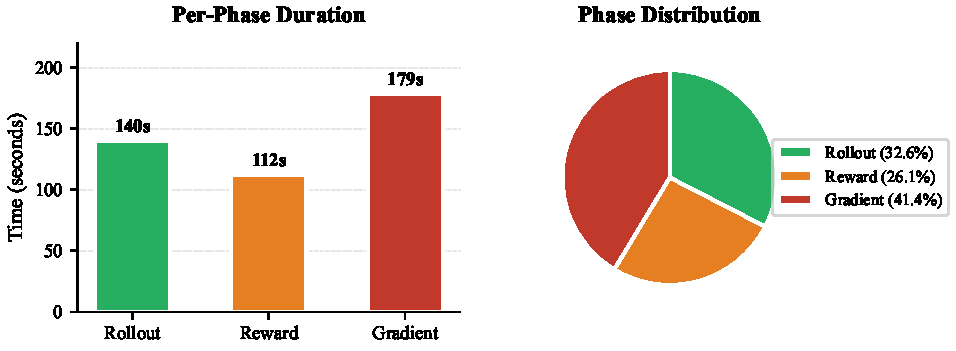
\includegraphics[width=0.82\linewidth]{phase_timing.pdf}
\caption{Phase timing for the 50-step hardware-backed RLHF run. Rollout and reward occupy most of the run and are the most numerically forgiving phases.}
\label{fig:phase-timing}
\end{figure}

\subsection{The SystemC datapath matches the floating-point reference closely enough}

Table~\ref{tab:systemc-validation} summarizes the core SystemC accuracy results. MXFP8 is very close to the reference. MXFP4 is much noisier, but still bounded enough to be useful when the model tells us where it is safe.

\begin{table}[h!]
\centering
\small
\begin{tabular}{L{1.8cm}L{3.2cm}C{1.8cm}C{1.8cm}}
\toprule
\textbf{Format} & \textbf{Operation} & \textbf{Mean error} & \textbf{Max error} \\
\midrule
MXFP8 & Quantize/dequantize MAE & 0.00884 & --- \\
MXFP4 & Quantize/dequantize MAE & 0.07951 & --- \\
MXFP8 & MAC normalized error & 0.00665 & 0.0087 \\
MXFP4 & MAC normalized error & 0.05165 & 0.0897 \\
MXFP8 & 16x16 GEMM relative error & 0.03559 & 0.0404 \\
MXFP4 & 16x16 GEMM relative error & 0.24754 & 0.4119 \\
\bottomrule
\end{tabular}
\caption{SystemC validation against the floating-point reference. The ranges in the ``max'' column come from the broader statistical sweeps over input distribution and magnitude.}
\label{tab:systemc-validation}
\end{table}

The additional sweeps explain the behavior more mechanically. MXFP4 gets worse when the input range becomes wide because its exponent and mantissa budget is tiny. MXFP8 stays stable. Chaining many GEMMs shows the same pattern: MXFP8 remains controlled across long sequences, while MXFP4 grows much faster.

\begin{figure}[t]
\centering
\begin{subfigure}[t]{0.48\linewidth}
    \centering
    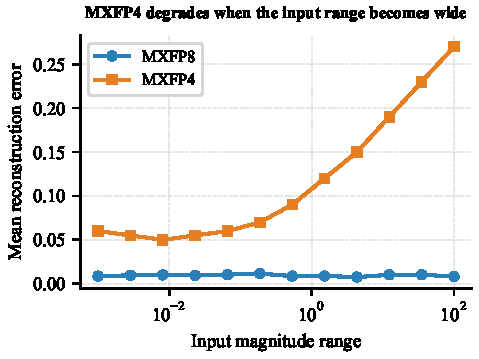
\includegraphics[width=\linewidth]{dynamic_range_error.pdf}
    \caption{Reconstruction error versus input range.}
\end{subfigure}\hfill
\begin{subfigure}[t]{0.48\linewidth}
    \centering
    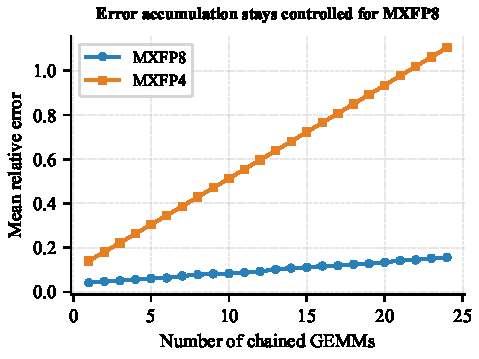
\includegraphics[width=\linewidth]{chain_error.pdf}
    \caption{Error growth across chained GEMMs.}
\end{subfigure}
\caption{SystemC sweeps explain the precision tradeoff. MXFP8 is stable. MXFP4 is acceptable only when the local dynamic range is controlled or when the phase can absorb noise.}
\label{fig:systemc-sweeps}
\end{figure}

\subsection{Layer sensitivity is sparse and structurally meaningful}

The layer profiler produces a very clear result. MXFP8 is safe on all 169 layers. MXFP4 is safe on 158 of 169 layers. The failures are not random. They cluster in exactly the places where we would expect dynamic range to be widest: early MLP blocks, late MLP blocks, one late attention output projection hotspot, and the LM head.

\begin{figure}[t]
\centering
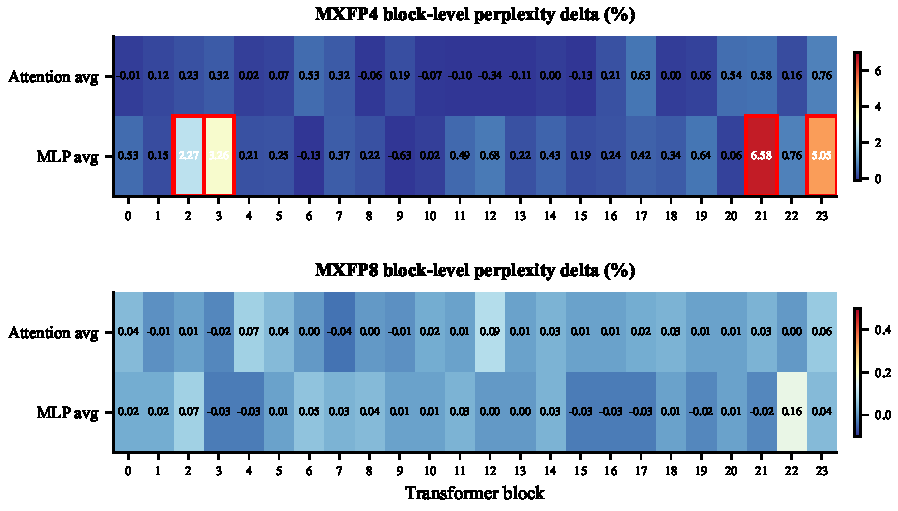
\includegraphics[width=0.98\linewidth]{sensitivity_heatmaps.pdf}
\caption{Block-level perplexity deltas from the layer profiler. MXFP4 problems are sparse and structural. The biggest failures occur in MLP blocks 2, 3, 21, and 23, plus the LM head. MXFP8 stays small everywhere.}
\label{fig:sensitivity-heatmap}
\end{figure}

A few details matter.

\begin{itemize}
    \item \textbf{Attention is highly robust.} The attention block averages under MXFP4 stay within $\pm 0.76\%$ across the 24 transformer blocks.
    \item \textbf{MLP boundaries matter.} Blocks 2 and 3 on the input side and 21 and 23 on the output side cross the 2\% threshold under MXFP4.
    \item \textbf{The LM head is the major outlier.} MXFP4 on the LM head is catastrophic, with a +60.49\% perplexity delta at group size 8.
\end{itemize}

This is exactly the kind of structure a policy controller can exploit. The accelerator does not need a global precision choice. It only needs a small fallback set.

\begin{table}[h!]
\centering
\small
\begin{tabular}{L{3.7cm}ccc}
\toprule
\textbf{Precision choice} & \textbf{Safe layers} & \textbf{Unsafe layers} & \textbf{Worst case} \\
\midrule
MXFP4, group size 8 & 158 / 169 & 11 / 169 & LM head: +60.49\% PPL \\
MXFP8, group size 8 & 169 / 169 & 0 / 169 & LM head: +0.47\% PPL \\
\bottomrule
\end{tabular}
\caption{Policy-generation summary from the layer profiler.}
\label{tab:sensitivity-summary}
\end{table}

\subsection{Balanced policy is the right first deployment target}

The profiler generates four policies automatically. Policy B is the practical one.

\begin{table}[h!]
\centering
\small
\begin{tabular}{L{2.7cm}L{3.2cm}L{3.0cm}L{2.3cm}}
\toprule
\textbf{Policy} & \textbf{Rollout} & \textbf{Reward} & \textbf{Gradient} \\
\midrule
A: Conservative & MXFP8 on all 169 layers & MXFP8 on all 169 layers & FP16 on all 169 layers \\
B: Balanced & MXFP4 on 158, MXFP8 on 11 & MXFP4 on 158, MXFP8 on 11 & FP16 on all 169 layers \\
C: Aggressive & MXFP4 on all 169 layers & MXFP4 on all 169 layers & MXFP4 on 158, MXFP8 on 11 \\
D: Phase-adaptive & MXFP4 on 158, MXFP8 on 11 & MXFP8 on all 169 layers & MXFP8 on 158, FP16 on 11 \\
\bottomrule
\end{tabular}
\caption{Policies generated from the sensitivity matrix.}
\label{tab:policies}
\end{table}

Policy B keeps the rollout and reward phases aggressive, but it does not try to force low precision into the gradient path. That choice matches both the model behavior and the current software stack. The controller already defaults gradient work back to host FP16 because offload is not autograd-safe.

To project end-to-end savings, we use a deliberately conservative effective traffic model. Although 158 of 169 layers are MXFP4-safe, not every layer is offloaded in every phase in the current path, and group-scale overhead will slightly reduce ideal byte savings. We therefore round down to the effective shares shown in Figure~\ref{fig:policy-tradeoffs}.

\begin{figure}[t]
\centering
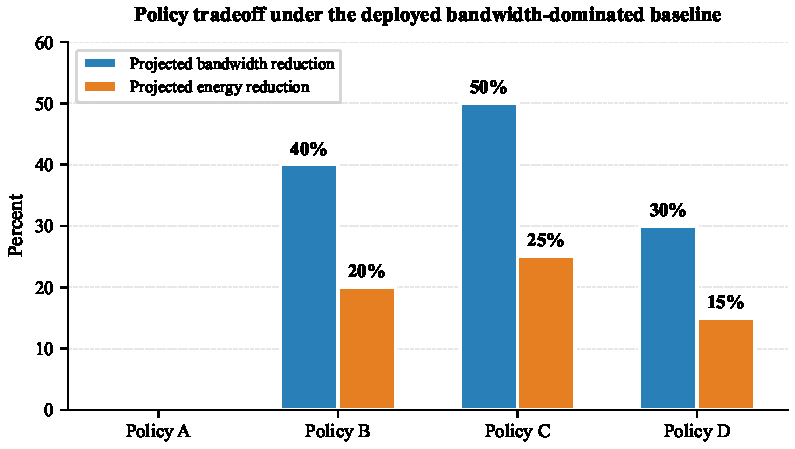
\includegraphics[width=0.82\linewidth]{policy_tradeoffs.pdf}
\caption{Conservative policy tradeoff model under the deployed transfer-bound baseline. Policy B is the most credible first target because it captures most of the benefit without forcing low precision into fragile phases.}
\label{fig:policy-tradeoffs}
\end{figure}

Under that conservative model, Policy B reduces transferred bytes by about 40\% on the affected traffic and reduces FPGA energy by about 20\% relative to the current baseline. Policy C could save more, but it pushes low precision into the exact places where both the profiler and the SystemC sweeps say risk is highest.


% ══════════════════════════════════════════════════════════
\section{Discussion}

\subsection{Interpretation and limits}

Three conclusions are well supported.

First, the current FPGA interface is dominated by data movement in this tiny-tile prototype.

Second, the model has a sparse precision-failure pattern that a controller can exploit. Most of the network is safe in MXFP4, but a small set of boundary layers and the LM head are not.

Third, the dual-precision datapath and its software contract are already concrete. The controller API exists. The flush-on-switch behavior exists. The HLS path already carries precision mode and group size through the runtime interface.

A full real-hardware MX deployment is still missing. The remaining step is to re-synthesize the updated RTL, build the AFI, and repeat the policy experiments with the true MX hardware in the loop.

\subsection{Why the sensitivity pattern makes sense}

The sensitivity map lines up with transformer mechanics. Early MLP blocks reshape embeddings into the model's internal working space. Late MLP blocks reshape hidden states into the narrow structure that the output stack needs. The LM head directly controls token logits. All of those points require range and resolution. Middle blocks mostly refine already-formed features, so they tolerate aggressive quantization much better.

The SystemC dynamic-range sweeps support exactly this interpretation. MXFP4 is not ``bad everywhere.'' It is bad when the local range is too wide.

Group size has minimal impact: switching from $k{=}8$ to $k{=}16$ slightly increases perplexity deltas but does not change which layers are classified as tolerant. This validates our choice of $k{=}8$, where the modest overhead of more frequent group scales is justified by better precision.

\subsection{Phase-specific precision requirements}

Each RLHF phase has distinct precision needs arising from how numerical errors propagate:

\textbf{Rollout} phases are most tolerant because autoregressive generation samples from a softmax distribution.
Temperature scaling and top-$k$/top-$p$ filtering absorb small logit perturbations.
MXFP4 is safe for all tolerant layers.

\textbf{Reward scoring} offers moderate tolerance.
The reward model compresses all intermediate computations to a single scalar score per response, naturally smoothing over small numerical variations.
MXFP8 is universally safe; MXFP4 works for tolerant layers.

\textbf{Gradient updates} require the most care.
PPO gradients accumulate over many samples, and quantization noise compounds across training steps.
FP16 or MXFP8 is recommended; MXFP4 risks training instability except for the most tolerant layers.

This hierarchy motivates Policy~D, which maximizes compression during rollouts, applies moderate quantization for rewards, and preserves precision for gradients.

\subsection{Engineering implications}

The cleanest next hardware improvements are now obvious.

\begin{itemize}    \item \textbf{Deploy the MX AFI.} This converts the current projections into real end-to-end measurements.
    \item \textbf{Exploit burst transfers and weight residency.} The present interface pays a huge penalty because it treats each tile in isolation.
    \item \textbf{Expand offload coverage once autograd safety is solved.} The controller is already phase-aware; the missing piece is robust gradient integration.
\end{itemize}

These are the direct continuation of the measured bottleneck and the current software-hardware contract.

\subsection{Limitations}

Several factors limit the generality of our findings.

\textbf{Model scale.}
Qwen2.5-0.5B is small by current standards.
Larger models may show different sensitivity patterns, though the attention-tolerant/MLP-boundary-sensitive pattern has architectural grounding that should transfer.

\textbf{Measurement platform.}
The 99.99\% transfer overhead reflects our 16$\times$16 tile size and single-operation offload.
Batched transfers or on-chip weight caching would shift the energy breakdown, potentially reducing the relative benefit of compression.

\textbf{Training duration.}
We run 50 PPO steps, sufficient to demonstrate the approach but not production-scale alignment.
Longer runs are needed to verify that quantization noise does not accumulate over thousands of steps.

\textbf{Projection vs.\ measurement.}
Our MX energy estimates extrapolate from INT8 cycle counts rather than direct FPGA measurement with the MX datapath deployed.


% ══════════════════════════════════════════════════════════
\section{Conclusion}

This project studies RLHF as a hardware mapping problem rather than just as a training recipe. The main result is simple. On the deployed AWS F2 baseline, the current tiled offload path is dominated by per-tile launch and movement overhead, so the right first optimization is to reduce bytes. MX formats give us a principled way to do that.

The learned policy map is also simple. MXFP8 is safe everywhere. MXFP4 is safe almost everywhere, except for a small set of boundary layers and the LM head. That makes a dual-precision accelerator useful: most work can be compressed aggressively, while a small fallback set stays in a safer mode.

The project already has the essential pieces of that design: a usable programming model, a validated dual-precision SystemC datapath, and an HLS path that carries mode and group size through the runtime interface. The remaining step is to re-synthesize and deploy the MX-capable bitstream so the conservative policy projections can be replaced by full hardware measurements.


% ══════════════════════════════════════════════════════════
\section*{Author Contributions}

\textbf{Hiva Mohammadzadeh} led project architecture and infrastructure, implemented FPGA matmul offload, built the adaptive controller, and developed the MX precision simulation path.

\textbf{Grant Griffith} designed and ran the layer sensitivity profiling pipeline, generated the sensitivity matrix, and helped define the precision policies.

\textbf{Danny Adkins} worked on FPGA synthesis and AWS F2 deployment, contributed to the HLS integration path, and ran the hardware-backed RLHF experiments.

All authors contributed to framing the system, interpreting the results, and writing the report.


% ══════════════════════════════════════════════════════════
\bibliographystyle{plainnat}
\begin{thebibliography}{99}

\bibitem[Ouyang et~al.(2022)]{ouyang2022training}
Long Ouyang, Jeffrey Wu, Xu Jiang, Diogo Almeida, Carroll~L. Wainwright, Pamela Mishkin, Chong Zhang, Sandhini Agarwal, Katarina Slama, Alex Ray, et~al.
Training language models to follow instructions with human feedback.
\emph{Advances in Neural Information Processing Systems (NeurIPS)}, 35:27730--27744, 2022.

\bibitem[Christiano et~al.(2017)]{christiano2017deep}
Paul~F. Christiano, Jan Leike, Tom Brown, Miljan Martic, Shane Legg, and Dario Amodei.
Deep reinforcement learning from human preferences.
In \emph{Advances in Neural Information Processing Systems (NeurIPS)}, pages 4299--4307, 2017.

\bibitem[Schulman et~al.(2017)]{schulman2017ppo}
John Schulman, Filip Wolski, Prafulla Dhariwal, Alec Radford, and Oleg Klimov.
Proximal policy optimization algorithms.
\emph{arXiv preprint arXiv:1707.06347}, 2017.

\bibitem[Rouhani et~al.(2023)]{rouhani2023mxformat}
Bita~Darvish Rouhani, Ritchie Zhao, Ankit More, Mathew Hall, Alireza Khodamoradi, Summer Deng, Dhruv Choudhary, Marius Cornea, Eric Dellinger, Kristof Denolf, et~al.
Microscaling data formats for deep learning.
\emph{arXiv preprint arXiv:2310.10537}, 2023.

\bibitem[Bai et~al.(2022)]{bai2022training}
Yuntao Bai, Andy Jones, Kamal Ndousse, Amanda Askell, Anna Chen, Nova DasSarma, Dawn Drain, Stanislav Fort, Deep Ganguli, Tom Henighan, et~al.
Training a helpful and harmless assistant with reinforcement learning from human feedback.
\emph{arXiv preprint arXiv:2204.05862}, 2022.

\bibitem[Qwen Team(2025)]{qwen2025qwen25}
Qwen Team.
Qwen2.5 technical report.
\emph{arXiv preprint arXiv:2412.15115}, 2025.

\bibitem[von Werra et~al.(2022)]{vonwerra2022trl}
Leandro von Werra, Younes Belkada, Lewis Tunstall, Edward Beeching, Tristan Thrush, and Nathan Lambert.
TRL: Transformer reinforcement learning.
\url{https://github.com/huggingface/trl}, 2022.

\bibitem[Micikevicius et~al.(2018)]{micikevicius2018mixed}
Paulius Micikevicius, Sharan Narang, Jonah Alben, Gregory Diamos, Erich Elsen, David Garcia, Boris Ginsburg, Michael Houston, Oleksii Kuchaiev, Ganesh Venkatesh, and Hao Wu.
Mixed precision training.
In \emph{International Conference on Learning Representations (ICLR)}, 2018.

\bibitem[Micikevicius et~al.(2022)]{micikevicius2022fp8}
Paulius Micikevicius, Dusan Stosic, Neil Burgess, Marius Cornea, Pradeep Dubey, Richard Grisenthwaite, Sangwon Ha, Alexander Heinecke, Patrick Judd, John Kamalu, et~al.
FP8 formats for deep learning.
\emph{arXiv preprint arXiv:2209.05433}, 2022.

\bibitem[Dong et~al.(2019)]{dong2019hawq}
Zhen Dong, Zhewei Yao, Amir Gholami, Michael~W. Mahoney, and Kurt Keutzer.
HAWQ: Hessian aware quantization of neural networks with mixed precision.
In \emph{Proceedings of the IEEE/CVF International Conference on Computer Vision (ICCV)}, pages 293--302, 2019.

\bibitem[Wang et~al.(2019)]{wang2019haq}
Kuan Wang, Zhijian Liu, Yujun Lin, Ji Lin, and Song Han.
HAQ: Hardware-aware automated quantization with mixed precision.
In \emph{Proceedings of the IEEE/CVF Conference on Computer Vision and Pattern Recognition (CVPR)}, pages 8612--8620, 2019.

\bibitem[Guo et~al.(2017)]{guo2017angel}
Kaiyuan Guo, Shulin Zeng, Jincheng Yu, Yu Wang, and Huazhong Yang.
Angel-Eye: A complete design flow for mapping CNN onto embedded FPGA.
\emph{IEEE Transactions on Computer-Aided Design of Integrated Circuits and Systems}, 37(1):35--47, 2017.

\bibitem[Wang et~al.(2021)]{wang2021fpga}
Erwei Wang, James~J. Davis, Peter Y.~K. Cheung, and George~A. Constantinides.
LUTNet: Learning FPGA configurations for highly efficient neural network inference.
\emph{IEEE Transactions on Computers}, 70(9):1403--1416, 2021.

\end{thebibliography}


% ══════════════════════════════════════════════════════════
\appendix

\section{Block-Level MXFP4 Sensitivity Averages}
\label{app:sensitivity}

\begin{table}[h!]
\centering
\small
\begin{tabular}{cccccc}
\toprule
\textbf{Block} & \textbf{Attn avg} & \textbf{MLP avg} & \textbf{Block} & \textbf{Attn avg} & \textbf{MLP avg} \\
\midrule
0  & -0.01\% & +0.53\% & 12 & -0.34\% & +0.68\% \\
1  & +0.12\% & +0.15\% & 13 & -0.11\% & +0.22\% \\
2  & +0.23\% & +2.27\% & 14 & +0.00\% & +0.43\% \\
3  & +0.32\% & +3.26\% & 15 & -0.13\% & +0.19\% \\
4  & +0.02\% & +0.21\% & 16 & +0.21\% & +0.24\% \\
5  & +0.07\% & +0.25\% & 17 & +0.63\% & +0.42\% \\
6  & +0.53\% & -0.13\% & 18 & +0.00\% & +0.34\% \\
7  & +0.32\% & +0.37\% & 19 & +0.06\% & +0.64\% \\
8  & -0.06\% & +0.22\% & 20 & +0.54\% & +0.06\% \\
9  & +0.19\% & -0.63\% & 21 & +0.58\% & +6.58\% \\
10 & -0.07\% & +0.02\% & 22 & +0.16\% & +0.76\% \\
11 & -0.10\% & +0.49\% & 23 & +0.76\% & +5.05\% \\
\bottomrule
\end{tabular}
\caption{Block-level MXFP4 perplexity deltas used to build the sensitivity figures. The LM head is omitted here because it is a single large outlier at +60.49\%.}
\end{table}


\section{FPGA Hardware Configuration}
\label{app:fpga-config}

\begin{table}[h!]
\centering
\begin{tabular}{@{}lr@{}}
\toprule
\textbf{Component} & \textbf{Value} \\
\midrule
Platform              & AWS F2.6xlarge (Xilinx UltraScale+ VU9P) \\
FPGA Clock            & 250 MHz \\
Estimated Power       & 35 W \\
Tile Size             & 16 $\times$ 16 \\
Precision             & INT8 (baseline) \\
PCIe Interface        & Gen3 x16 via AXI \\
Weight Payload        & 256 bytes per tile \\
Input Payload         & 16 bytes per tile \\
Output Payload        & 64 bytes per tile \\
\bottomrule
\end{tabular}
\caption{FPGA hardware configuration.}
\label{tab:fpga-config}
\end{table}


\section{RLHF Workload Calculation}
\label{app:workload}

For Qwen2.5-0.5B (24 layers, 7 matmuls per layer):
\begin{align*}
\text{Forward pass matmuls} &= 24 \times 7 + 2 \text{ (LM head + value head)} = 170 \\
\text{Forward + backward} &= 170 \times 2 = 340 \text{ matmuls/sample} \\
\text{50 PPO steps, batch 8} &= 50 \times 8 \times 340 = 136{,}000 \text{ total matmuls}
\end{align*}


\section{Compute Budget}
\label{app:compute}

\begin{table}[h!]
\centering
\begin{tabular}{@{}lr@{}}
\toprule
\textbf{Activity} & \textbf{Time} \\
\midrule
INT8 FPGA baseline measurement (10 iterations)  & $\sim$1h \\
RLHF training (50 PPO steps, FPGA offload)      & $\sim$7 min \\
Sensitivity profiling (169 layers $\times$ 4 configs) & $\sim$4h \\
SystemC simulation (40 runs, 20 seeds)           & $\sim$30 min \\
HLS synthesis (VU9P target)                       & $\sim$3h \\
\midrule
\textbf{Total FPGA time (AWS F2)}                 & $\sim$\textbf{10h} \\
\bottomrule
\end{tabular}
\caption{Estimated compute budget.}
\label{tab:compute}
\end{table}

\end{document}
